% !TEX root = ../thesis.tex
%*******************************************************************************
%********************************** Fourth Chapter *****************************
%*******************************************************************************
% **************************** Define Graphics Path **************************
\ifpdf
    \graphicspath{{Chapter4/Figs/Raster/}{Chapter4/Figs/PDF/}{Chapter4/Figs/}}
\else
    \graphicspath{{Chapter4/Figs/Vector/}{Chapter4/Figs/}}
\fi

\chapter{Abusive Language Detection}\label{chap:detection}

\section{Typology of Abuse - Published} \zw{Ask committee if this can be used, has now been published in another person's thesis}
In \cite{Waseem:2017}, we consider the implications of the current state of abusive language detection. In \cite{Davidson:2017} and \cite{Schmidt:2017}, clear misunderstandings of the term ``hate speech'' occur, considering both a legal, gender studies and critical race studies point of view. To effect this, we worked on a paper to emphasize  and encourage researchers to focus on the manner in which the abuse occurs rather than the kind of abuse occurring, as focusing overly on the type of abuse will inevitably lead to potential overlaps between multiple tasks in the general topic of abusive language detection.

In the work, we propose that abusive language will exist in the following forms (please see table \ref{tab:typology} for more examples):
\begin{itemize}
  \item{Directed Abuse\\In this case the abuse is aimed a particular individual or entity.}
  \item{Generalized Abuse\\Is the abuse generalized, it seeks to attack a large group of people, for instance by use of stereotyping an oppressed minority.}
  \item{Explicit Abuse\\Explicit Abuse may be explicit for instance by using bad words (slurs amongst other things).}
  \item{Implicit Abuse\\Implicit Abuse is abusive comments that seek to use alliterations, similes, and euphemisms amongst others to communicate abusive content. An example of this, is referring to refugees from Syria in terms of waves and streams, where the implicit connotations are that they are overrunning Europeans and must be stopped, lest we all ``drown''.}
\end{itemize}

% \begin{table*}[ht]
% \centering
% \begin{tabular}{p{\textwidth/30}|p{0.45\textwidth}|p{0.45\textwidth}}
%   & \textit{Explicit}    & \textit{Implicit} \\\hline
%     \multirow{4}{*}{\rotatebox[origin=c]{90}{\textit{Directed}}}    &   {\scriptsize``Go kill yourself'',  ``You're a sad little f*ck'' \citep{Hee:2015a}}, \newline {\scriptsize ``@User shut yo beaner ass up sp*c and hop your f*ggot ass back across the border little n*gga''  \citep{Davidson:2017}}, \newline {\scriptsize ``Youre one of the ugliest b*tches Ive ever fucking seen'' \citep{Kontostathis:2013}}. & {\scriptsize ``Hey Brendan, you look gorgeous today. What beauty salon did you visit?'' \citep{dinakar2012common}, \newline ``(((@User))) and what is your job?  Writing cuck articles and slurping Google balls?  \#Dumbgoogles'' \citep{Hine:2016},\newline  ``you're intelligence is so breathtaking!!!!!!'' \citep{dinakar2011modeling}}\\\hline
%   \multirow{5}{*}{\rotatebox[origin=c]{90}{\textit{Generalized}}} & {\scriptsize``I am surprised they reported on this crap who cares about another dead n*gger?'', ``300 missiles are cool! Love to see um launched into Tel Aviv! Kill all the g*ys there!'' \citep{Nobata:2016}, \newline ``So an 11 year old n*gger girl killed herself over my tweets? \^ \_ \^\ thats another n*gger off the streets!!'' \citep{Kwok:2013}}. & {\scriptsize``Totally fed up with the way this country has turned into a haven for terrorists. Send them all back home.'' \citep{burnap2015cyber}, \newline ``Gas the skypes'' \citep{magu2017detecting}, \newline ``most of them come north and are good at just mowing lawns'' \citep{dinakar2011modeling}} \\
% \end{tabular}
%   \caption{Typology of abusive language \citep{Waseem:2017}.}
% \label{tab:typology}
% \end{table*}
%
in Table \ref{tab:typology} we see a mapping of the categories proposed and how they may interact.

\section{Challenges of the task}

\zw{Show here how poorly models generalise to other datasets; refer back to racial biases in datasets}

% This project was a collaboration between Zeerak Waseem, James Thorne (University of Sheffield), and Joachim Bingel (University of Copenhagen)\footnote{This project was the result of equal contribution from all authors.}.\vspace{5mm}
%
%
% This project sought to investigate the applicability of Multi-Task Learning for abusive language detection. The overarching aim of the project was to investigate the hypothesis that disparate data sets annotated for different kinds of abusive language in which the demographics writing the abuse can are different can be utilized for a unified model for abusive language detection.
%
% We applied data from \cite{Waseem-Hovy:2016,Waseem:2016} and \cite{Davidson:2017}. The tweets collected by \cite{Waseem-Hovy:2016} and \cite{Waseem:2016} were collected without a specific demographic selected whereas \cite{Davidson:2017} collected tweets that originated from the United States of America. Given that these differences meant that the datasets contained documents from several different demographic groups, each with their own understandings of bias and abuse we sought to investigate whether it was possible to utilize the distinct groups to improve detection of abusive language.
%
% To investigate this we built classifiers trained on a single data set\footnote{\cite{Waseem-Hovy:2016} and \cite{Waseem:2016} are concatenated into a single data set as they are collected from the same initial scrape }, the concatenation of all data sets, and a multi-task learning configuration in which multiple models are trained simultaneously.
%
% \begin{table}[hbt]
% \centering
% \caption{Comparison of test-set performance of within-domain and out-of-domain datasets using models trained only on one dataset (first four rows), models trained by concatenating both datasets (middle two rows), and using both datasets in a multi-task learning environment (final four rows). For each training regime, we compare using Bag-of-Words (BoW), the Average of Subword Embeddings (Emb) and both (B+E) as features for each tweet. Key: (R)acism, (S)exism, (H)ate-Speech, (O)ffensive, (N)either. Datasets: Davidson \cite{Davidson:2017}, Waseem\cite{Waseem:2016}/Waseem-Hovy\cite{Waseem-Hovy:2016} (W/W+H)}
% \label{tab:results}
%
% \begin{tabular}{|c|c||c||c|c|c|c||c|c|c|c|} 
% \hline
% \multicolumn{2}{|c||}{\textbf{Training Objective}} & \multirow{3}{*}{\textbf{Feats}} & %\multicolumn{8}{|c|}{\textbf{$F_1$-Scores of Predictions on Test Sets}}  \\
% \cline{1-2}
% \cline{4-11}
% \multirow{2}{*}{\textbf{Primary}} & \multirow{2}{*}{\textbf{Aux}} & & %\multicolumn{4}{|c||}{\textbf{W/W+H}} & \multicolumn{4}{|c|}
% {\textbf{Davidson}} \\
% \cline{4-11}
% & & & R & S & N & Avg & H & O & N & Avg\\
% \hline
% \hline
% W/W+H & - & BoW & 0.70 & 0.65 & 0.88 & 0.82 & 0.00 & 0.64 & 0.42 & 0.57 \\
% W/W+H & - & Emb & 0.30 & 0.42 & 0.85 & 0.71 & 0.01 & 0.04 & 0.29 & 0.08 \\
% W/W+H & - & B+E & 0.00 & 0.00 & 0.82 & 0.57 & 0.00 & 0.00 & 0.29 & 0.05\\
% \hline
% Davidson & - & BoW & 0.22 & 0.29 & 0.69 & 0.56 & 0.32 & 0.94 & 0.84 & 0.89 \\
% Davidson & - & Emb  & 0.00 & 0.32 & 0.60 & 0.48 & 0.19 & 0.92 & 0.69 & 0.84 \\
% Davidson & - & B+E & 0.25 & 0.33 & 0.70 & 0.58 & 0.39  & 0.82 & 0.94 & 0.89 \\
% \hline
% \hline
% Both & - & BoW & 0.21 & 0.54 & 0.81 & 0.70 & 0.20 & 0.92 & 0.77 & 0.86 \\
% Both & - & Emb & 0.21 & 0.45 & 0.76 & 0.64 & 0.05 & 0.90 & 0.64 & 0.80\\
% Both & - & B+E & 0.17 & 0.53 & 0.81 & 0.69 & 0.31 & 0.92 & 0.77 & 0.86 \\
% \hline
% \hline
% W/W+H & Davidson & BoW & 0.64 & 0.63 & 0.87 & 0.80 & 0.39 & 0.94 & 0.84 & 0.89 \\
% W/W+H & Davidson & Emb & 0.32 & 0.50 & 0.84 & 0.72 & 0.10 & 0.91 & 0.64 & 0.82 \\
% W/W+H & Davidson & B+E & 0.51 & 0.53 & 0.86 & 0.75 & 0.16 & 0.93 & 0.78 & 0.86 \\
% \hline
% Davidson & W/W+H & BoW & 0.66 & 0.62 & 0.86 & 0.79 & 0.37 & 0.94 & 0.83 & 0.89 \\
% Davidson & W/W+H & Emb & 0.39 & 0.49 & 0.84 & 0.73 & 0.09 & 0.91 & 0.62 & 0.81 \\
% Davidson & W/W+H & B+E & 0.60 & 0.57 & 0.85 & 0.77 & 0.14 & 0.93 & 0.78 & 0.86 \\
% \hline
% \end{tabular}
% \end{table}
%
% We find that while we did not see improvements over the concatenated models, strong improvements were made over simply using a single training set. Importantly, we see that using multi-task learning we achieve similar performance to concatenating a data set, which allows for further research to continue with this setting using more data sets that may give related signals to abusive language detection.
%
% \section{Reframing Content Moderation in the Context of Care - In review}
%
% This project is conducted in collaboration with Nanna Bonde Thylstrup from Copenhagen Businesss School.
%
% In this project we seek to reframe the logics of content moderation with the logics of content moderation. While content moderation has often been framed in the context of censorship and removal, we here propose to view content moderation in a lens of community care, in which impacted communities are brought to the center of the problem, rather than the peripheral casualties of content mdoeration. This work, in the context of computer science research, allows us to rethink how computational models for content moderation may be built to allow for an intersectional feminist approach to automated content moderation through returning agency to the affected communities.
% In the context of social scientific thought on content moderation, we seek here to describe (internal) processes and motivations of content moderators at smaller companies. We develop our empirical basis through semi-structured interviews with content moderators from two different companies which engage with the dissemination of sound and webpages, respectively.\vspace{5mm}
%
% Through our interviews, we find that the process of content moderation shows striking similarities with nine characterstics of infrastructures as described by \cite{Graham-Thrift:2007} from the work of \cite{Star:1999} and \cite{Star-Ruhleder:1996}. The similarities are expressed in terms of content moderation acting as cultural filters which raise question about pollutive behavior \cite{Douglas:2015}, seeking to separate the harmful from the harmless content.
%
% \section{Fair Fake News Detection - In Draft}
%
% In this project we aim to extend the method of \cite{Agarwal:2018} to text classification and examine its usefulness for deriving fair classifiers detecting fake news. We use the dataset published by \cite{Wang:2017} which contains statements in the general area of political conversations. For each statement the dataset contains multiple properties including party affiliation, name of the speaker, venue of the statement, subjects of the statement, state the speaker is in, and their job title. In this project we set the protected attribute to be political affiliation, as ones political affiliation should not have an impact on the prediction of the classifier. The method proposed by \cite{Agarwal:2018} is an iterative process of training constrained models in which the constraints updated each time a model has been trained. The updated contraints are computed as a function of violation of the selected fairness criteria.\vspace{5mm}
%
% \subsection{Data}
% The \cite{Wang:2017} dataset contains $12$K statements labelled with 6 classes obtained from Politifact,\footnote{Politifact is a professional fact checking organization.} along with data for each document detailing their party affiliation, job title, the venue of the statement,\footnote{Venue here refers to the type of place the statement was made, e.g. 'social media', 'rally', and 'radio interview'} the name of the speaker, the subjects of the statement, and the state the speaker is in. To estimate if \cite{Agarwal:2018} can be applied, we change the prediction task to a binary classification task by collapsing the labels 'pants-on-fire', 'false', and 'barely-true' to our positive class and 'true', 'mostly-true' and 'half-true' to our negative class. Further, we restrict the data set to only statements which are made by people with declared political affiliations, specifically we consider Democrats and Republicans from the United States of America. Our functioning dataset thus consists of $9.8$K statements which are split into $7,855$ for training, $992$ for validation, and $990$ in our test set.
%
% \subsection{Selecting Protected Attributes}
% In our selection of which meta-data category to use as the protected attribute, we consider gender (as derived from names) and political affiliation. We limit our gender-tagged data to be limited to people who have declared party affiliations to ensure that we can uniquely and accurately identify gender. For both datasets we train a classifier to predict the protected attribute using unigrams. The results of predicting gender (omitted) show that a classifier trained to predict gender only slightly outperforms a random choice model, this suggests that a gender bias may not be expressed strongly in the dataset. On the other hand, a model trained to predict political affiliation using unigrams achieves a reasonable result (see \autoref{tab:feat_exploration}) suggesting that a model for fake news detection {\textit may} correlations between political affiliations and fake news. For our methods, we use demographic parity as our fairness criteria. Demographic Parity states that the predictions of a model must be statistically independent of the protected attribute. We choose this as we wish for a complete independence of political affiliation and predictions of fake news.
%
% \begin{table*}[ht]
% \resizebox{\textwidth}{!}{%
% \begin{tabular}{l|l|lll}
%   Feature Set                               & Feature                                                             & Accuracy   & Precision & Recall \\\hline
%   \multirow{2}{*}{n-grams}                  & Unigrams                                                            & 63,13      & 0.62      & 0.63   \\
%                                             & Unigrams + Bigrams                                                  & \bf{64.04} & 0.63      & \bf{0.64} \\\hline
%    LIWC                                     & LIWC                                                                & 59.59      & 0.36      & 0.60   \\\hline
%    Sentiment                                & Sentiment                                                           & 56.66      & 0.36      & 0.60   \\\hline
%   \multirow{4}{*}{Dependency Feats}         & Arc                                                                 & 62.32      & 0.52      & 0.51   \\
%                                             & Children                                                            & 62.72      & 0.61      & 0.63   \\
%                                             & Head                                                                & 61.31      & 0.60      & 0.61   \\
%                                             & Arc Count                                                           & 59.39      & 0.58      & 0.59   \\
%                                             & Dependency Features                                                 & 60.70      & 0.60      & 0.61   \\\hline
%   \multirow{3}{*}{Reading Ease Feats}       & Dale-Chall                                                          & 59.49      & 0.54      & 0.59   \\
%                                             & Sentence Length                                                     & 59.79      & \bf{0.76} & 0.60   \\
%                                             & Avg. Word Length                                                    & 59.39      & 0.46      & 0.59   \\
%                                             & Reading Ease Features                                               & 59.09      & 0.52      & 0.59   \\\hline
%   \multirow{8}{*}{Feature Combinations}     & Reading Ease Feats + Unigram                                        & 63.63      & 0.63      & \bf{0.64}\\
%                                             & Reading Ease Feats + Unigram + Bigram                               & 62.92      & 0.62      & 0.63   \\
%                                             & Dependency Feats + Unigram                                          & 61.01      & 0.60      & 0.61   \\
%                                             & Dependency Feats + Unigram + Bigram                                 & 61.71      & 0.61      & 0.62   \\
%                                             & Unigrams + LIWC + Sentiment + Dependency Feats + Reading Ease Feats & 61.31      & 0.61      & 0.61   \\
%                                             & LIWC + Unigram                                                      & 63.33      & 0.62      & 0.63   \\
%                                             & LIWC + Unigrams + Bigrams                                           & 61.51      & 0.60      & 0.62   \\
%                                             & All Features                                                        & 62.02      & 0.61      & 0.62
% \end{tabular}%
% }
% \caption{Feature Exploration using Logistic Regression}
% \label{tab:feat_exploration}
% \end{table*}
%
% \subsection{Defining Fairness}
%
% In a consideration of what it means for a classifier to be fair, we consider error rates and accuracies for each class. The aim for a fair classifier is then to minimise differences between error rates for each protected attribute.
% Error rates are computed by considering all instances of misclassification for each category of the protected attributes
% \begin{equation}
%   \left|\dfrac{1}{|Y|}\sum_{i\in X} \mathbf{1}\{y_i \neq \hat{y_i} \land y_i = \text{republican}\} - \dfrac{1}{|Y|}\sum_{i\in X} \mathbf{1}\{y_i \neq \hat{y_i} \land y_i = \text{democrat}\}\right|
%   \label{eq:err_rate}
% \end{equation}
% where $C$ is the set of classes and $X$ is the set of documents that are being predicted on, and $Y$ is the set of labels, and $y_i = \text{democrat}$ is replaced by 'republican' to compute the error rate for republicans. We then take the absolute value for differences between the error rate for each protected attribute.
%
% Similarly we compute the difference in accuracy for each class by replacing the $\neq$ with $=$ in \autoref{eq:err_rate}.
%
% \subsection{Building a Fair Classifier}
% The method proposed by \cite{Agarwal:2018} views computation of a fair classifier as a two player game that seeks a $\nu$-approximate equillibrium, where a saddlepoint is computed such that neither player can gain more than $\nu$ by changing their choice. The classifier is constrained by a set of linear constraints which represent the protected attributes. Formally, we can define our constraints as
% \begin{equation}
%   \min_{Q\in\Delta} \widehat{err}(Q) \text{ subject to } \bm{M\mu}(Q) \leq \mathbf{c}
%   \label{eq:constraint}
% \end{equation}
% where $\mathbf{c}$ and $\mathbf{M}$ express the linear constraints as a matrix and vector, $Q$ is a randomized classifier, and $\bm{\mu}$ is a conditional moment.\vspace{5mm}
%
% The algorithm computes the saddlepoint through an iterative process in which a classifier is trained on a set of linear constraints which are expressed in terms of lagrangian multipliers. In each iteration, we initially update the lagrangian multipliers for each of the $\mathcal{K}$ constraints. Using the updated lagrangian multipliers, we compute a classifier $h$ which allows us to compute the actions of our two players (classifiers) $\\hat{Q}$ and $\hat{\lambda}$. In effect, the lagrangian multipliers allow us to modify our feature weights as a function of the constraint violationof the previous iteration. In each iteration, we store the classifier which has the smallest constraint violation, using its constraint violation to update the values of our lagrangian multipliers.
%
% The result of this computation is a set of classifiers which iteratively are more fair, as the constraints of the models are updated.\vspace{5mm}
%
% While the method may be applied to linear and non-linear classifiers alike, we focus on linear classifiers to allow us for considering the changes in feature weights.
%
% \paragraph{Blind Classifier} We also apply a weak form of Fairness through unawareness \cite{Grgic-Hlaca}, which seeks to remove the influence of features that are indicative of the protected class - notably \cite{Grgic-Hlaca} show that reducing or removing the influence of indicative features does not guarantee that the classifier produces fair predictions. In our approach, we compute a classifier to predict the protected attribute, identify the $400$ most indicative features ($200$ for each class), and train a classifier to predict our main task, fake news, while we remove access to the $400$ most indicative features for the protected attributes. We use a logistic regression model for our blind classifier.
%
% \subsection{Model Selection}
%
% For all unfair and fair models, with the exception of the blind classifier, we use three different models: Logistic Regression (LR), Support Vector Machines (SVM), and Random Forests (RF). For each classifier type, we initially perform a grid-search over the models parameters on the vanilla fake news detection problem, the best parameters for each model are then applied to all versions of it.
%
% \paragraph{Baselines} As the \cite{Wang:2017} paper experimented with a multi-class classifier, we first train a multi-class classifier to ensure that we obtain the same results, then we retrain the classifier using binary labels. Due to the low accuracy of the binary classifier, we show experiment with different features (see \autoref{tab:feat_exploration}, we note that all feature sets were evaluated using a Logistic Regression classifier) which show that unigrams obtain a competitive baseline with little improvement in classification scores by using more advanced feature sets. Therefore we use unigrams for all of our classifiers.
%
% \begin{table*}[ht]
% \resizebox{\textwidth}{!}{%
% \begin{tabular}{l|l|lll}
%   Feature Set                              & Feature                                                             & Accuracy   & Precision & Recall \\\hline
%   \multirow{2}{*}{n-grams}                 & Unigrams                                                            & 63,13      & 0.62      & 0.63   \\
%                                            & Unigrams + Bigrams                                                  & \bf{64.04} & 0.63      & \bf{0.64} \\\hline
%    LIWC                                    & LIWC                                                                & 59.59      & 0.36      & 0.60   \\\hline
%    Sentiment                               & Sentiment                                                           & 56.66      & 0.36      & 0.60   \\\hline
%   \multirow{4}{*}{Dependency Feats}        & Arc                                                                 & 62.32      & 0.52      & 0.51   \\
%                                            & Children                                                            & 62.72      & 0.61      & 0.63   \\
%                                            & Head                                                                & 61.31      & 0.60      & 0.61   \\
%                                            & Arc Count                                                           & 59.39      & 0.58      & 0.59   \\
%                                            & Dependency Features                                                 & 60.70      & 0.60      & 0.61   \\\hline
%   \multirow{3}{*}{Reading Ease Feats}      & Dale-Chall                                                          & 59.49      & 0.54      & 0.59   \\
%                                            & Sentence Length                                                     & 59.79      & \bf{0.76} & 0.60   \\
%                                            & Avg. Word Length                                                    & 59.39      & 0.46      & 0.59   \\
%                                            & Reading Ease Features                                               & 59.09      & 0.52      & 0.59   \\\hline
%   \multirow{8}{*}{Feature Combinations}    & Reading Ease Feats + Unigram                                        & 63.63      & 0.63      & \bf{0.64}\\
%                                            & Reading Ease Feats + Unigram + Bigram                               & 62.92      & 0.62      & 0.63   \\
%                                            & Dependency Feats + Unigram                                          & 61.01      & 0.60      & 0.61   \\
%                                            & Dependency Feats + Unigram + Bigram                                 & 61.71      & 0.61      & 0.62   \\
%                                            & Unigrams + LIWC + Sentiment + Dependency Feats + Reading Ease Feats & 61.31      & 0.61      & 0.61   \\
%                                            & LIWC + Unigram                                                      & 63.33      & 0.62      & 0.63   \\
%                                            & LIWC + Unigrams + Bigrams                                           & 61.51      & 0.60      & 0.62   \\
%                                            & All Features                                                        & 62.02      & 0.61      & 0.62
% \end{tabular}%
% }
% \caption{Feature Exploration using Logistic Regression}
% \label{tab:feat_exploration}
% \end{table*}
%
% In addition to the the baseline computed using the binary version of the \cite{Wang:2017} classifier, we also compute an unfair SVM and random forest classifier to serve as additional baselines. Finally, we show baselines on predicting party affiliation using a model trained to predict party affiliation and unfair models trained to predict fake news where we use the heuristic that all predictions of ``Fake'' map to ``republican'' and all predictions of ``True'' map to ``democrat''. See \autoref{tab:baselines} for all baselines.
%
% \begin{table*}[ht]
%  \resizebox{\textwidth}{!}{
% \begin{tabular}{lllllllll}
%                                                 & Accuracy (overall) & Precision & Recall & F1-score & Accuracy (Class0) & Accuracy (Class1) & Error Rate (Class0) & Error Rate (Class1) \\
% Unfair LR (Fake News - all data)                & 0.6305             & 0.63      & 0.63   & 0.63     & 0.4982            & 0.7317            & 0.1519              & 0.2174              \\
% Unfair SVM (Fake News - all data)               & 0.6024             & 0.60      & 0.60   & 0.60     & 0.5215            & 0.6643            & 0.1901              & 0.2073              \\
% Unfair RF (Fake News - all data)                & 0.6250             & 0.62      & 0.63   & 0.60     & 0.3669            & 0.8225            & 0.1005              & 0.2743              \\
% Random Baseline (Fake News - all data)          & 0.5003             & 0.51      & 0.50   & 0.50     & 0.4946            & 0.5048            & 0.2805              & 0.2190              \\
% Unfair LR (Fake News - dem/rep)                 & 0.6313             & 0.62      & 0.63   & 0.62     & 0.4525            & 0.75254237        & 0.1474              & 0.2212              \\
% Unfair SVM (Fake News - dem/rep)                & 0.6020             & 0.60      & 0.60   & 0.60     & 0.5175            & 0.6593            & 0.2030              & 0.1949              \\
% Unfair RF (Fake News - dem/rep)                 & 0.6272             & 0.61      & 0.63   & 0.61     & 0.3750            & 0.7983            & 0.1202              & 0.2525              \\
% Random Baseline (Fake News - dem/rep)           & 0.5040             & 0.52      & 0.50   & 0.51     & 0.5               & 0.5067            & 0.2939              & 0.2020              \\
% Unfair Pretrained LR (Dem/rep prediction)       & 0.5202             & 0.57      & 0.52   & 0.51     &                   &                   &                     &                     \\
% Unfair Pretrained SVM (dem/rep prediction)      & 0.5292             & 0.56      & 0.53   & 0.53     &                   &                   &                     &                     \\
% Unfair Pretrained RF (dem/rep prediction)       & 0.5060             & 0.58      & 0.51   & 0.48     &                   &                   &                     &                     \\
% Random Baseline (Dem/rep prediction)            & 0.4717             & 0.49      & 0.47   & 0.48     & 0.4672            & 0.4780            & 0.2161              & 0.312               \\
%
% \end{tabular}}
% \caption{Baselines}
% \label{tab:baselines}
% \end{table*}
%
% \subsection{Results}
%
% In \autoref{tab:results} we see the that by applying our blind classifier, we improve the classification accuracy to $0.84$ with a a sharp decrease in error rates compared to the unfair Logistic Regression model. Considering then our fair Logistic Regression model, we see that the classification error increases, however if we consider the relative error computed, there is a slight decrease in the error rate.\footnote{We are still considering which exact error metric to use, so we are leaving the error rates in the table as is for now.}
%
% \begin{table*}[ht]
% \resizebox{\textwidth}{!}{
% \begin{tabular}{lllllllll}
%                                                 & Accuracy (overall) & Precision & Recall & F1-score & Accuracy (Class0) & Accuracy (Class1) & Error Rate (Class0) & Error Rate (Class1) \\
% Blind (dem/rep)                                 & 0.7745             & 0.78      & 0.77   & 0.77     & 0.6318            & 0.88211           & 0.0672              & 0.1582              \\
% LR (Dem/rep prediction)                         & 0.6676             & 0.66      & 0.67   & 0.66     & 0.8086            & 0.4682            & 0.2202              & 0.1121              \\
% SVM (Dem/rep prediction)                        & 0.6434             & 0.64      & 0.64   & 0.64     & 0.6965            & 0.5682            & 0.1787              & 0.1777              \\
% RF (Dem/rep prediction)                         & 0.6131             & 0.60      & 0.61   & 0.59     & 0.8172            & 0.3243            & 0.2898              & 0.1070              \\
% Fair Fake News LR (dem/rep)                     & 0.5252             & 0.52      & 0.53   & 0.52     & 0.36              & 0.6372            & 0.2161              & 0.2585              \\
% Fair Fake News SVM                              & 0.4808             & 0.49      & 0.48   & 0.48     & 0.39              & 0.5423            & 0.2727              & 0.2464              \\
% Fair Fake News RF                               & 0.5909             & 0.58      & 0.59   & 0.58     & 0.415             & 0.7101            & 0.1727              & 0.2363              \\
% Fair Pretrained LR (Dem/rep prediction)         & 0.3575             & 0.38      & 0.36   & 0.35     &                   &                   &                     &                     \\
% Fair Pretrained SVM (Dem/rep prediction)        & 0.3676             & 0.39      & 0.37   & 0.37     &                   &                   &                     &                     \\
% Fair Pretrained RF (Dem/rep prediction)         & 0.4959             & 0.54      & 0.50   & 0.49     &                   &                   &                     &
% \end{tabular}}
% \caption{Results of our models}
% \label{tab:results}
% \end{table*}
% \end{rotatebox}
%
% Turning our attention to using the fair fake news models to predict party affiliation, we see that in the process of learning a fair fake news classifier, the modification of features has resulted in a classifier which negatively associates republicans with fake news. As the unfair model learns that features which indicate fake news also indicate republicans, this negative association falls in line with our expectations of the model's performance. In \autoref{fig:feature_dev} we show the development of 10 features which are strongly predictive of republicans and democrats, respectively.
%
% \begin{figure*}
%   \centering
%   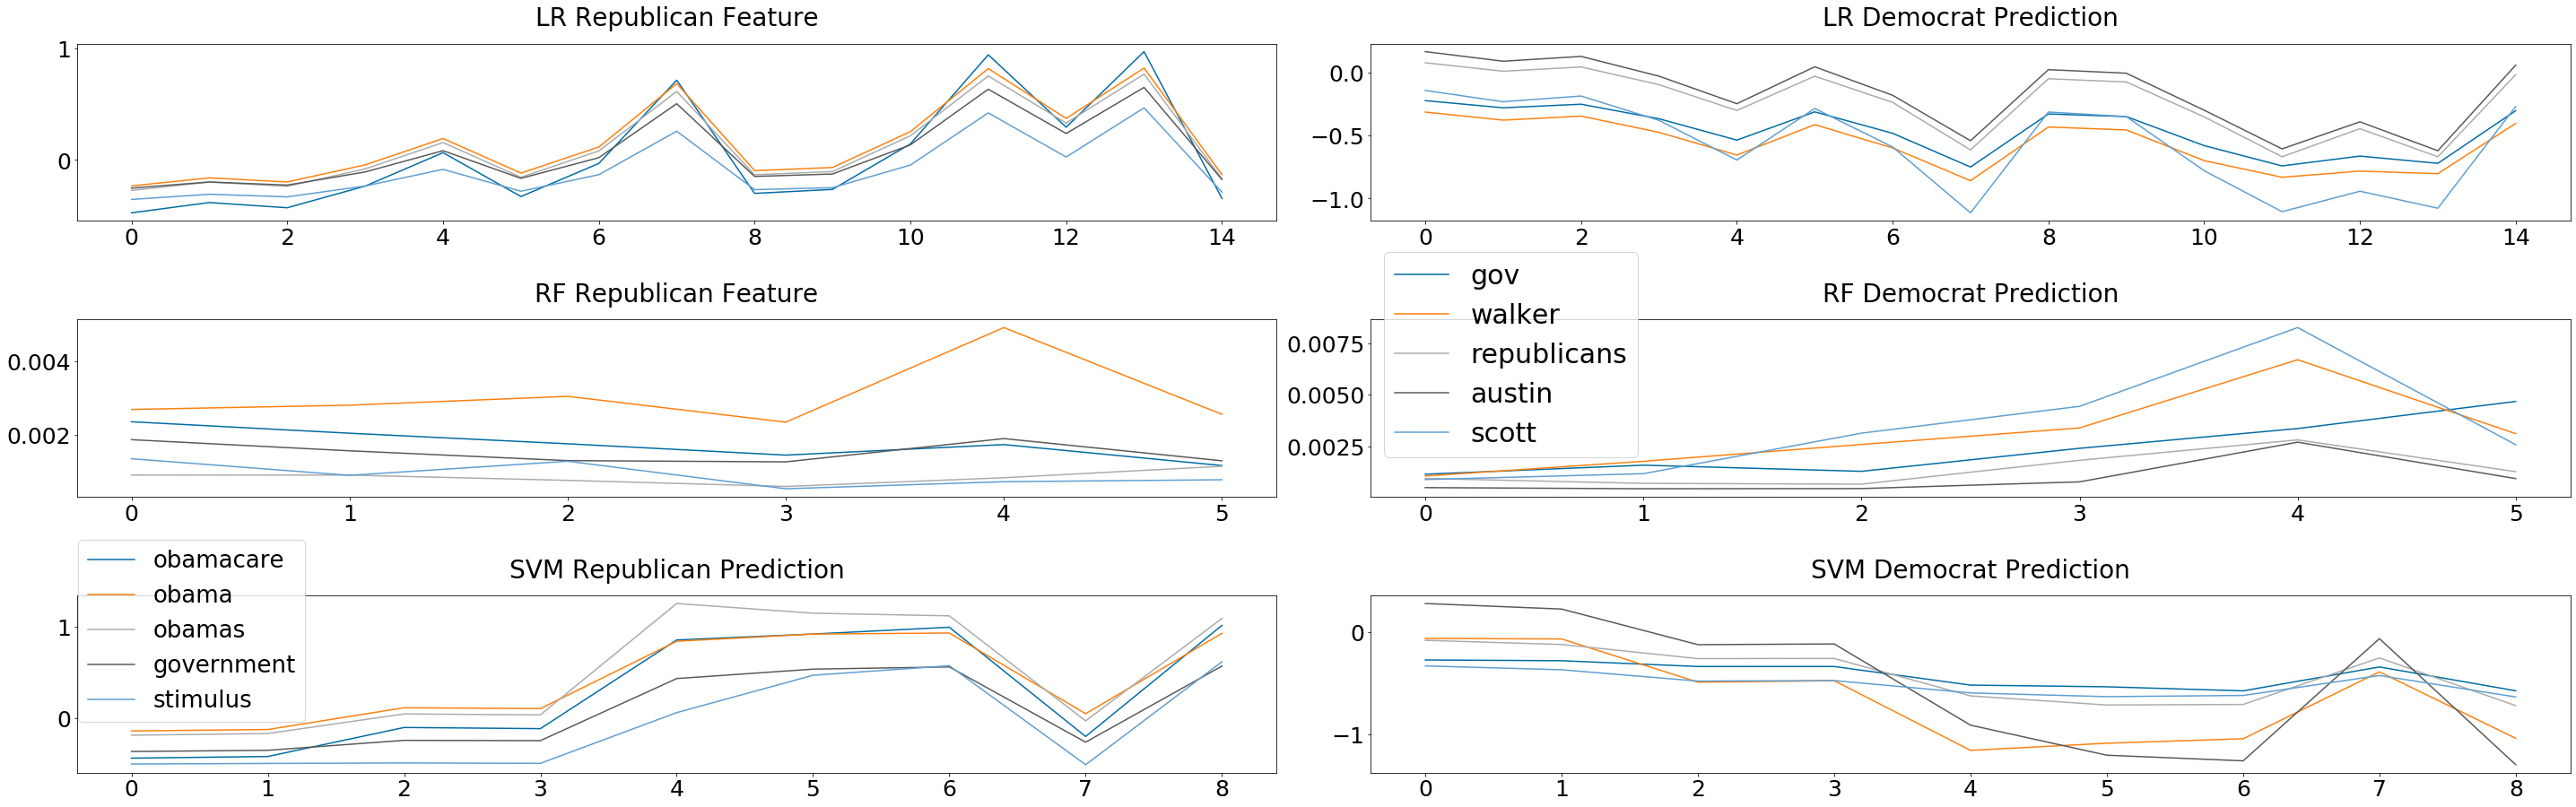
\includegraphics[width=\textwidth]{feature_dev.png}
%   \caption{Development of 10 most predictive features for predicting party affiliation.}
%   \label{fig:feature_dev}
% \end{figure*}
%
% Based on our results we can conclude that the dataset proposed by \cite{Wang:2017} contains bias against republicans and that intelligent feature selection may yield similar results to modifying a classifier for fairness, with a boost to the classification performance obtained by disallowing the classifier access to biased terms.
%
% \section{Critical NLP - Draft}
%
% This work is in undertaken in collaboration with Maya Indira Ganesh, Leuphana University of L{\¨u}neburg. In this early draft, we see a conversation between an doctoral student in NLP and a doctoral student in Science and Technology Studies (STS) on the need for critical thought in NLP, how research in NLP on topics such as abuse and hate speech can ignore populations affected by NLP tools and further marginalize them. In our work, we take a step back from the implementations and the specific task and seek to ask how NLP tools can be inclusive of communities afflicted by them and how they can speak to, rather than about the communities that are affected. Importantly, we also situate the researcher - highlighting that for some problems, the experiences, identities, knowledge, and biases that the researchers bring into their approach to the tasks. For instance, for abusive language there is a marked lack of African-American researchers devoted to the problem - this has likely had an influence on the fact that a number of datasets for abusive language all exhibit biases against African American Vernacular English \citep{Davidson:2019,Sap:2019}. We provide concrete considerations for researchers when they work on tasks which may influence communities to which they do not belong.
%
% \section{Summary}
%
% In this chapter, we have briefly introduced the projects which have lead to publication, the papers have been drafted or are in review at this point. Please see Appendix \ref{appendix:published} for more detail of published papers and \autoref{appendix:draft} for more detail on draft and review versions of papers.
